%Version 3 December 2023
% See section 11 of the User Manual for version history
%
%%%%%%%%%%%%%%%%%%%%%%%%%%%%%%%%%%%%%%%%%%%%%%%%%%%%%%%%%%%%%%%%%%%%%%
%%                                                                 %%
%% Please do not use \input{...} to include other tex files.       %%
%% Submit your LaTeX manuscript as one .tex document.              %%
%%                                                                 %%
%% All additional figures and files should be attached             %%
%% separately and not embedded in the \TeX\ document itself.       %%
%%                                                                 %%
%%%%%%%%%%%%%%%%%%%%%%%%%%%%%%%%%%%%%%%%%%%%%%%%%%%%%%%%%%%%%%%%%%%%%

%%\documentclass[referee,sn-basic]{sn-jnl}% referee option is meant for double line spacing

%%=======================================================%%
%% to print line numbers in the margin use lineno option %%
%%=======================================================%%

%%\documentclass[lineno,sn-basic]{sn-jnl}% Basic Springer Nature Reference Style/Chemistry Reference Style

%%======================================================%%
%% to compile with pdflatex/xelatex use pdflatex option %%
%%======================================================%%

%%\documentclass[pdflatex,sn-basic]{sn-jnl}% Basic Springer Nature Reference Style/Chemistry Reference Style


%%Note: the following reference styles support Namedate and Numbered referencing. By default the style follows the most common style. To switch between the options you can add or remove “Numbered” in the optional parenthesis. 
%%The option is available for: sn-basic.bst, sn-vancouver.bst, sn-chicago.bst%  
 
%%\documentclass[pdflatex,sn-nature]{sn-jnl}% Style for submissions to Nature Portfolio journals
%%\documentclass[pdflatex,sn-basic]{sn-jnl}% Basic Springer Nature Reference Style/Chemistry Reference Style
\documentclass[pdflatex,sn-mathphys-num]{sn-jnl}% Math and Physical Sciences Numbered Reference Style 
%%\documentclass[pdflatex,sn-mathphys-ay]{sn-jnl}% Math and Physical Sciences Author Year Reference Style
%%\documentclass[pdflatex,sn-aps]{sn-jnl}% American Physical Society (APS) Reference Style
%%\documentclass[pdflatex,sn-vancouver,Numbered]{sn-jnl}% Vancouver Reference Style
%%\documentclass[pdflatex,sn-apa]{sn-jnl}% APA Reference Style 
%%\documentclass[pdflatex,sn-chicago]{sn-jnl}% Chicago-based Humanities Reference Style

%%%% Standard Packages
%%<additional latex packages if required can be included here>

\usepackage{graphicx}%
\usepackage{multirow}%
\usepackage{amsmath,amssymb,amsfonts}%
\usepackage{amsthm}%
\usepackage{mathrsfs}%
\usepackage[title]{appendix}%
\usepackage{xcolor}%
\usepackage{textcomp}%
\usepackage{manyfoot}%
\usepackage{booktabs}%
\usepackage{algorithm}%
\usepackage{algorithmicx}%
\usepackage{algpseudocode}%
\usepackage{listings}%
\usepackage{bbm}%

%%%%

%%%%%=============================================================================%%%%
%%%%  Remarks: This template is provided to aid authors with the preparation
%%%%  of original research articles intended for submission to journals published 
%%%%  by Springer Nature. The guidance has been prepared in partnership with 
%%%%  production teams to conform to Springer Nature technical requirements. 
%%%%  Editorial and presentation requirements differ among journal portfolios and 
%%%%  research disciplines. You may find sections in this template are irrelevant 
%%%%  to your work and are empowered to omit any such section if allowed by the 
%%%%  journal you intend to submit to. The submission guidelines and policies 
%%%%  of the journal take precedence. A detailed User Manual is available in the 
%%%%  template package for technical guidance.
%%%%%=============================================================================%%%%

%% as per the requirement new theorem styles can be included as shown below
\theoremstyle{thmstyleone}%
\newtheorem{theorem}{Theorem}%  meant for continuous numbers
%%\newtheorem{theorem}{Theorem}[section]% meant for sectionwise numbers
%% optional argument [theorem] produces theorem numbering sequence instead of independent numbers for Proposition
\newtheorem{proposition}[theorem]{Proposition}% 
%%\newtheorem{proposition}{Proposition}% to get separate numbers for theorem and proposition etc.

\theoremstyle{thmstyletwo}%
\newtheorem{example}{Example}%
\newtheorem{remark}{Remark}%

\theoremstyle{thmstylethree}%
\newtheorem{definition}{Definition}%

\raggedbottom
%%\unnumbered% uncomment this for unnumbered level heads

\begin{document}

\title[Article Title]{MyRAG: Advancing Retrieval-Augmented Generation with Comparative Analysis of Standard RAG, ColBERT Reranking, and RAPTOR Architectures}

%%=============================================================%%
%% GivenName	-> \fnm{Joergen W.}
%% Particle	-> \spfx{van der} -> surname prefix
%% FamilyName	-> \sur{Ploeg}
%% Suffix	-> \sfx{IV}
%% \author*[1,2]{\fnm{Joergen W.} \spfx{van der} \sur{Ploeg} 
%%  \sfx{IV}}\email{iauthor@gmail.com}
%%=============================================================%%

\author*[1]{\fnm{Meet} \sur{Daxini}}\email{meet.daxini@gwu.edu}


\affil*[1]{\orgdiv{Department of Data Science}, \orgname{The George Washington University}, \state{Washington DC}, \country{USA}}


%%==================================%%
%% Sample for unstructured abstract %%
%%==================================%%

\abstract{Retrieval-Augmented Generation (RAG) has emerged as a powerful paradigm for providing personalized, relevant, and current information to user queries by combining large language models (LLMs) with external retrieval modules. This paper presents \textit{MyRAG}, an open source code that unifies and compares different state-of-the-art RAG architectures and retrieval techniques. This paper explores embeddings, vector databases, and advanced retrieval approaches, including ColBERT (Contextualized Late Interaction over Bidirectional Encoder Representations from Transformers) for contrastive reranking and RAPTOR (Recursive Abstractive Processing for Tree-Organized Retrieval) for hierarchical summarization-based retrieval. By evaluating different datasets, it demonstrates how different configurations impact retrieval accuracy and downstream QA performance. The results offer insights into optimizing RAG pipelines, guiding both practitioners and researchers toward more efficient and effective retrieval-augmented generation.}

%%================================%%
%% Sample for structured abstract %%
%%================================%%

% \abstract{\textbf{Purpose:} The abstract serves both as a general introduction to the topic and as a brief, non-technical summary of the main results and their implications. The abstract must not include subheadings (unless expressly permitted in the journal's Instructions to Authors), equations or citations. As a guide the abstract should not exceed 200 words. Most journals do not set a hard limit however authors are advised to check the author instructions for the journal they are submitting to.
% 
% \textbf{Methods:} The abstract serves both as a general introduction to the topic and as a brief, non-technical summary of the main results and their implications. The abstract must not include subheadings (unless expressly permitted in the journal's Instructions to Authors), equations or citations. As a guide the abstract should not exceed 200 words. Most journals do not set a hard limit however authors are advised to check the author instructions for the journal they are submitting to.
% 
% \textbf{Results:} The abstract serves both as a general introduction to the topic and as a brief, non-technical summary of the main results and their implications. The abstract must not include subheadings (unless expressly permitted in the journal's Instructions to Authors), equations or citations. As a guide the abstract should not exceed 200 words. Most journals do not set a hard limit however authors are advised to check the author instructions for the journal they are submitting to.
% 
% \textbf{Conclusion:} The abstract serves both as a general introduction to the topic and as a brief, non-technical summary of the main results and their implications. The abstract must not include subheadings (unless expressly permitted in the journal's Instructions to Authors), equations or citations. As a guide the abstract should not exceed 200 words. Most journals do not set a hard limit however authors are advised to check the author instructions for the journal they are submitting to.}

\keywords{Retrieval-Augmented Generation, RAG, ColBERT, RAPTOR, Natural Language Processing}


%%\pacs[JEL Classification]{D8, H51}

%%\pacs[MSC Classification]{35A01, 65L10, 65L12, 65L20, 65L70}

\maketitle

\newpage

\section{Introduction}\label{sec1}

The exponential growth of digital information has increased the demand for intelligent systems that can efficiently retrieve relevant context and answer complex questions. Large Language Models (LLMs) often possess extensive parametric knowledge, but may lack reliable, up-to-date information. Retrieval-Augmented Generation (RAG) has gained prominence as a solution to this challenge, bridging large-scale language understanding with external retrieval components to produce more grounded and accurate responses \cite{lewis2020retrieval, guu2020realm}.

In RAG pipelines, as illustrated in Figure \ref{fig:standard_rag_flow},  the LLM accesses external knowledge sources, retrieving relevant documents or chunks to augment its prompt. This approach enhances the model’s factual accuracy, reduces hallucinations, and updates knowledge without retraining the entire model. As the sizes of the context window continue to expand \cite{liu2023lost}, it is increasingly practical to provide LLMs with larger and more diverse sets of the retrieved context.

\begin{figure}[h]
    \centering
    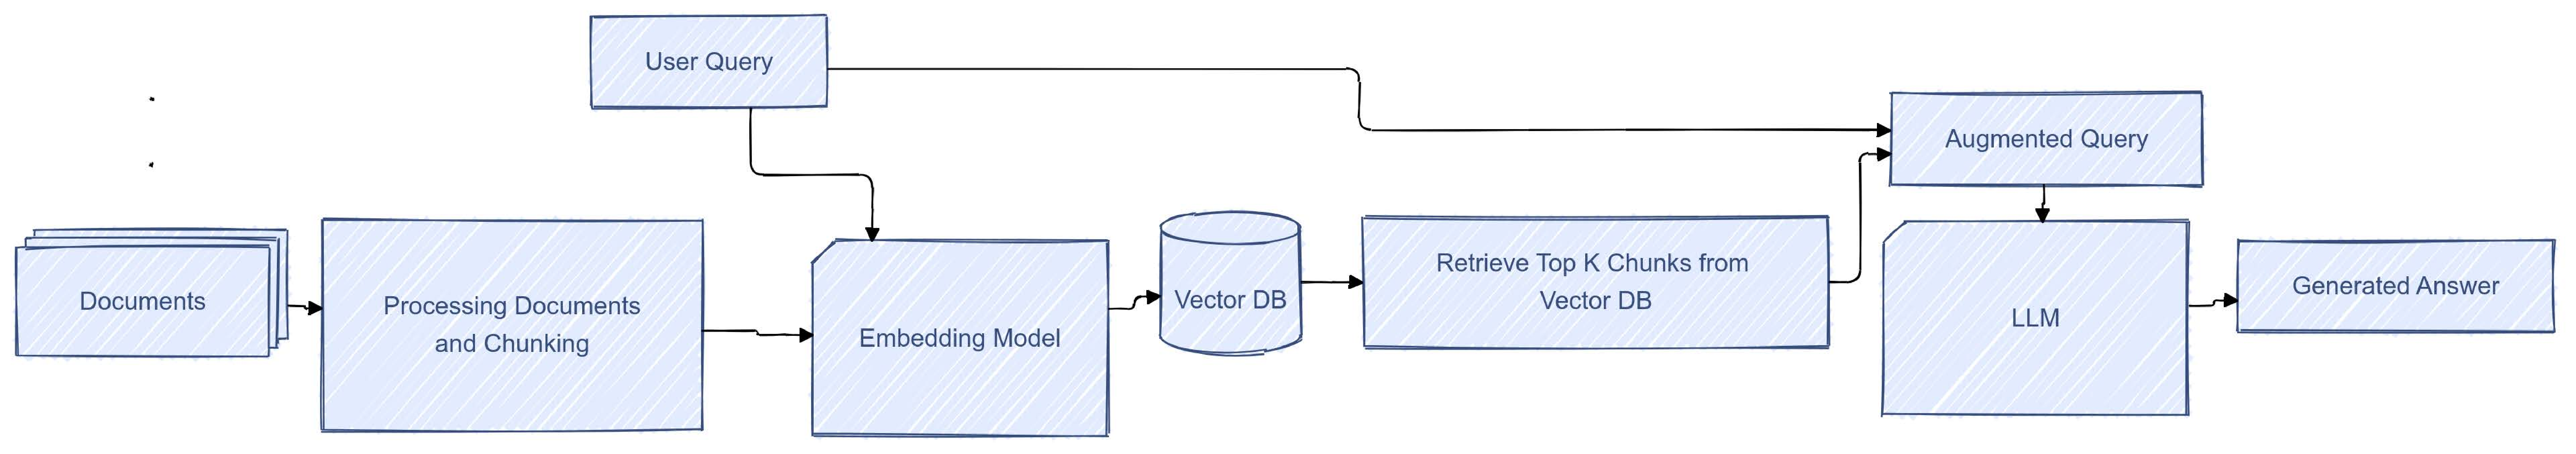
\includegraphics[width=\linewidth]{StandardRag.pdf} 
    \caption{Flow chart illustrating the standard RAG pipeline.}
    \label{fig:standard_rag_flow}
\end{figure}


Yet, not all retrieval pipelines are created equal. Various embedding models, databases (like graph, vector, etc), and advanced retrieval techniques can be combined to form a RAG system. For instance, This paper explores How Standard Rag with ColBERT \cite{khattab2020colbert} re-ranking can refine retrieved documents, while the RAPTOR architecture \cite{wu2021recursively, raptor2024} organizes and summarizes documents hierarchically. Understanding the trade-offs between these methods is key to building robust and scalable RAG systems.

This paper introduces \textit{MyRAG}, an open source code designed to compare multiple retrieval and augmented generation strategies systematically. We evaluate embeddings, vector stores, and advanced retrieval enhancements like ColBERT re-ranking and RAPTOR summarization, applying them on the BioASQ \cite{bioasq2023} and Hugging Face Document QA datasets \cite{huggingface2024docqa}. Our experiments aim to provide a clearer understanding of how these components influence retrieval accuracy and end-to-end QA performance.
 

\section{Problem Statement}\label{sec2}

While the Massive Text Embedding Benchmark (MTEB) \cite{muennighoff2022mteb} provides valuable insights into embedding model performance across diverse tasks, there remains a critical need for comprehensive evaluation of end-to-end RAG architectures. The current landscape lacks:

\begin{enumerate}
    \item \textbf{Architecture-Specific Evaluation:} Unlike MTEB's focus on embedding quality, MyRAG provides systematic comparison of different RAG architectures - ColBERT reranking \cite{khattab2020colbert}, and RAPTOR hierarchical retrieval \cite{wu2021recursively, raptor2024} - using consistent datasets, metrics, vector stores (Chroma and DeepLake) and quantization strategies.
    
    \item \textbf{Resource-Conscious Assessment:} MyRAG evaluates both 8-bit quantized and full-precision versions of popular embedding models addressing practical deployment considerations not covered by MTEB's leaderboard.
    
    \item \textbf{Intuitive Real-World Metrics:} MyRAG introduces straightforward measures beyond MTEB's technical metrics:
    \begin{itemize}
        \item Correct/Partial/Incorrect answer classification
        \item Multi-document per question retrieval accuracy 
        \item Response generation quality with context
        \item Resource utilization across architectures
    \end{itemize}
\end{enumerate}

Through this comprehensive evaluation framework, MyRAG helps practitioners select optimal combinations of embedding models (guided by MTEB's leaderboard), retrieval architectures, and implementation approaches. The framework supports both detailed technical assessment and simple, interpretable metrics that organizations need to optimize their RAG deployments across use cases and resource constraints. By offering comparison of standard RAG, ColBERT reranking, and RAPTOR approaches on multtiple datasets, MyRAG provides actionable insights for building more effective retrieval-augmented generation systems.


\textit{MyRAG} addresses this need by providing an open source code that enables direct, end-to-end comparisons of RAG approaches. By incorporating multiple embedding models, vector databases, reranking strategy (ColBERT), and hierarchical retrieval architecture (RAPTOR), \textit{MyRAG} provides a clear, cohesive platform for empirical evaluation. This approach ensures that even non-experts can understand performance trade-offs through accessible and practical metrics, ultimately guiding practitioners and researchers toward more optimal and tailored RAG solutions.

\section{Methodology}\label{sec3}
MyRAG builds on the works by offering a unified platform to compare multiple embedding models, vector stores, and rag architectures including ColBERT and RAPTOR and provides a flexible pipeline to switch between embedding models, vector stores, and retrieval techniques. Key components include:

\subsection{Parsing Documents and Chunking}\label{subsec3.1}


MyRAG employs a robust text processing pipeline for document parsing and chunking, leveraging the \texttt{RecursiveCharacterTextSplitter} from LangChain python library. This method enables efficient handling of large textual data by splitting documents into manageable, contextually coherent chunks while preserving overlap for improved information retrieval.

\subsection{Embedding Models}\label{subsec3.2}

MyRAG supports a range of embedding models that are integrated 
 with AWS Bedrock and Hugging Face Transformers. These models translate textual inputs into high-dimensional vector representations, which serve as the foundation for semantic similarity-based retrieval.

\begin{itemize}
    \item \textbf{Hugging Face-Based Models:} Models such as NV-Embed-v2, Stella 1.5B, MXBai Large, and all-MiniLM-L6-v2 are supported via the Hugging Face Transformers library. The implementation includes automatic device management (CPU/CUDA), 8-bit quantization support, and configurable device mapping for efficient resource utilization.

    \item \textbf{Amazon Bedrock Integration:} The Amazon Titan embedding model is accessed through AWS Bedrock's runtime client api. 
\end{itemize}

These embedding strategies form a core component of MyRAG's retrieval workflow. By evaluating models across benchmark datasets, it becomes possible to determine which embedding configurations yield the best balance of retrieval accuracy, computational efficiency, and downstream QA performance.

\subsection{Vector Databases}\label{subsec3.3}

MyRAG integrates support for Chroma and DeepLake, two vector databases specifically designed to optimize similarity search. These databases leverage \textbf{Hierarchical Navigable Small World (HNSW)} indices \cite{malkov2016efficient}, which are highly efficient for approximate nearest neighbor search. HNSW organizes vectors in a spatial domain into hierarchical clusters, enabling scalable similarity comparisons. In addition to HNSW indices, both Chroma and DeepLake support similarity metrics like cosine and \(L_2\) distance, making them versatile for a wide range of use cases. Furthermore, these vector databases handle rich metadata alongside the vector representations, allowing for more nuanced queries and contextual filtering. These features collectively enhance the performance and scalability of retrieval pipelines within the MyRAG framework.


\subsection{LLMs} \label{subsec3.4}
MyRAG supports integration with both AWS Bedrock and Hugging Face python library Transformers-based models for text generation. These Large Language Models (LLMs) serve as the backbone of the retrieval-augmented generation workflow, consuming retrieved documents as context and producing coherent, contextually grounded responses. 

\begin{itemize}
    \item \textbf{AWS Bedrock LLMs:} Anthropic's Claude variants are accessed through AWS Bedrock's runtime client API. 
    
    \item \textbf{Hugging Face Transformers LLMs:} Meta-Llama-3-8B-Instruct and in future other open source model support will be added
\end{itemize}


\subsection{ColBERT Reranking} \label{subsec3.5}
ColBERT \cite{khattab2020colbert} provides a reranking framework that refines retrieval results by comparing query tokens against all tokens in candidate documents, rather than relying on a single vector embedding per document. Unlike traditional embeddings, which compress each document into a single vector, ColBERT applies a late interaction mechanism to handle token-level embeddings. The standard document scoring process in RAG, as illustrated in Figure \ref{fig:standard_doc_scoring}, demonstrates how documents are typically scored based on similarity to the query, with the top k documents retrieved based on their overall scores. In contrast, ColBERT scoring operates differently, as described here and illustrated in Figure \ref{fig:colbert}. Instead of a single score for each document, ColBERT computes similarities between individual query tokens and token embeddings in the documents, ensuring that finer contextual alignments are captured.


\begin{figure}[h]
	\centering
	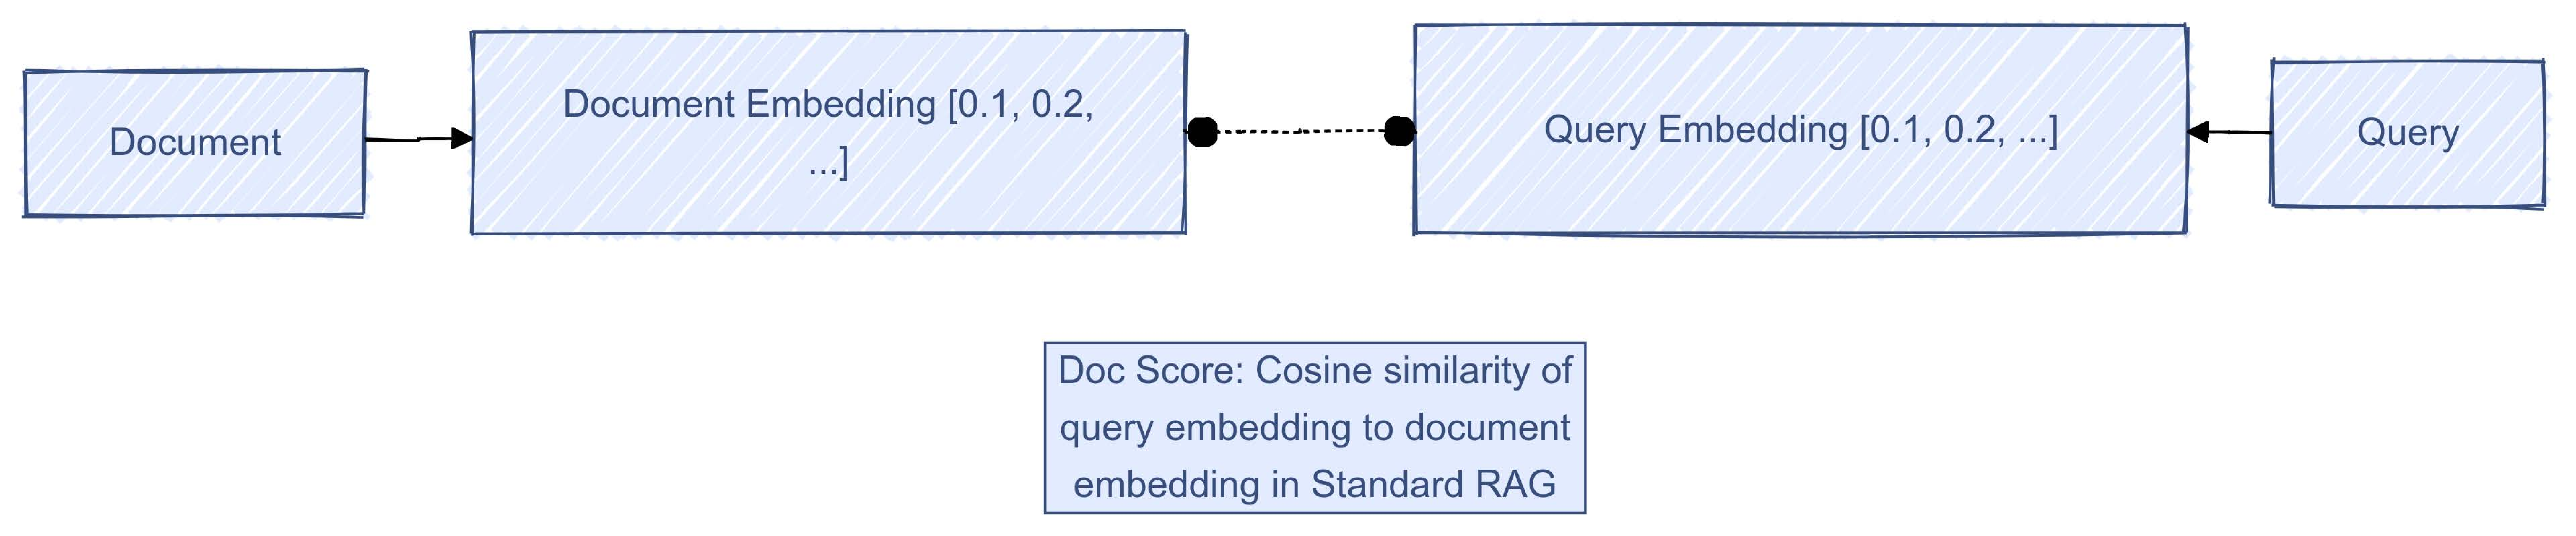
\includegraphics[width=\linewidth]{StandardRAGDocumentScoring.pdf}
	\caption{Flow chart of Standard RAG Embeddings Document Scoring within vector database}
	\label{fig:standard_doc_scoring}
\end{figure}

\begin{figure}[h]
	\centering
	\includegraphics[width=\linewidth]{Colbert.pdf}
	\caption{Flow chart of ColBert Document Scoring}
	\label{fig:colbert}
\end{figure}

\begin{figure}[h]
	\centering
	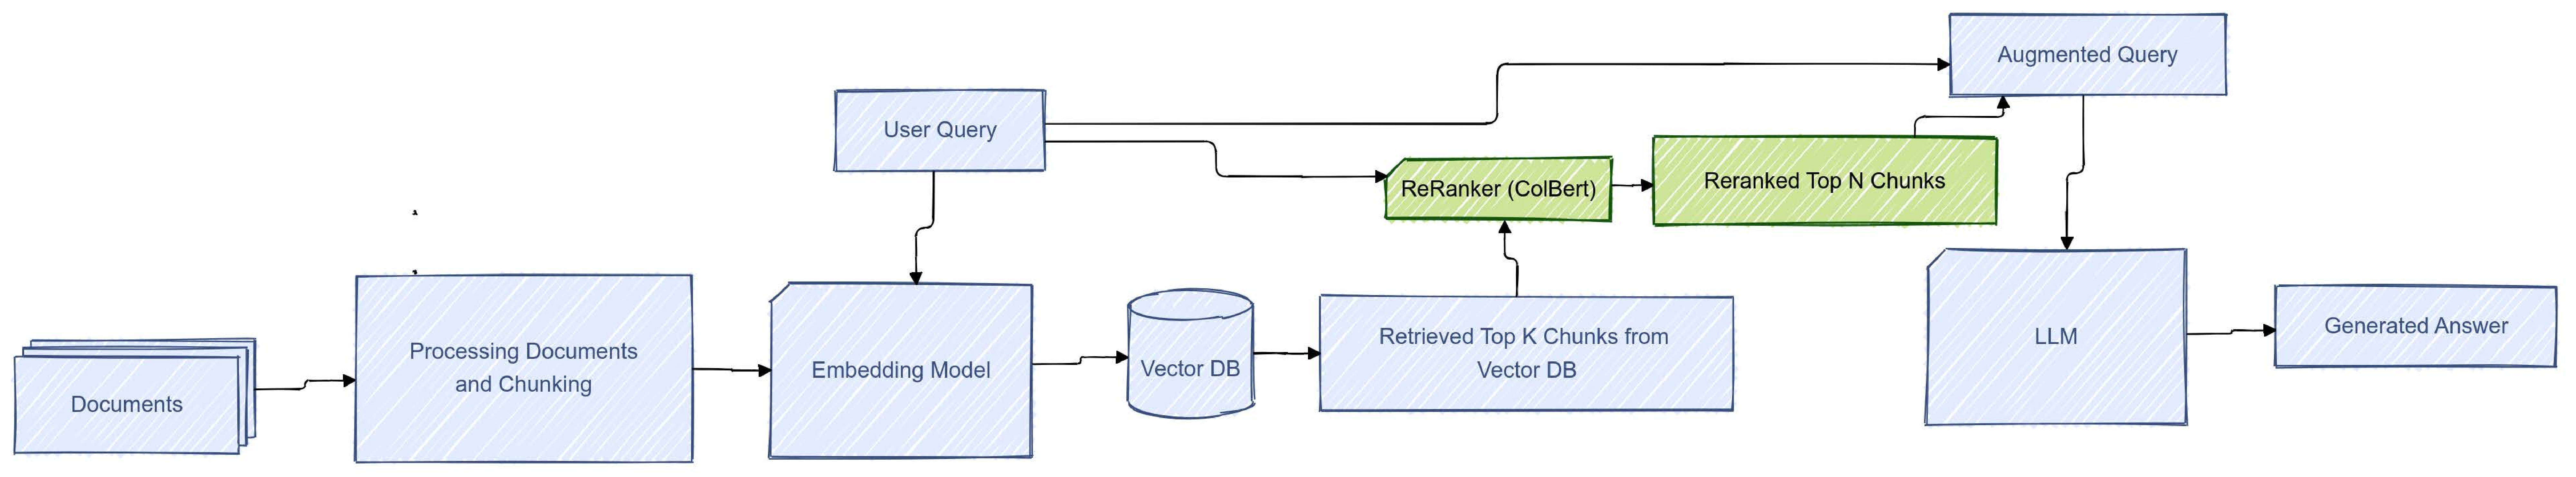
\includegraphics[width=\linewidth]{StandardRagWithReRanking.pdf}
	\caption{Flow chart of Standard Rag with ColBert Reranking as integrated in MyRag}
	\label{fig:reranking_rag}
\end{figure}

Figure \ref{fig:reranking_rag} outlines how ColBERT reranking is integrated within the MyRAG system, demonstrating how the reranked results from ColBERT feed into the subsequent retrieval-augmented generation process. The implementation in MyRAG leverages the RAGatouille python library to integrate ColBERT v2.0 model for the re-ranking step following the initial retrieval process. After retrieving a candidate set of documents, the RAGatouille-based ColBERT implementation scores each document based on fine-grained token alignments with the query. These fine-grained comparisons enable the system to re-prioritize documents that contain subtle but crucial semantic clues.


\subsection{RAPTOR: Recursive Abstractive Processing for Tree-Organized Retrieval} \label{subsec3.6}
RAPTOR \cite{wu2021recursively, raptor2024} organizes documents into a hierarchical retrieval structure via recursive clustering and summarization. It embeds documents using a chosen embedding model and applies UMAP for dimensionality reduction. A Gaussian Mixture Model (GMM) guided by the Bayesian Information Criterion (BIC) then clusters documents, automatically determining an optimal number of clusters (up to 50). Each cluster is recursively summarized at multiple levels, with each level’s summaries serving as inputs for higher-level abstraction. 

This hierarchical process, as illustrated in Figure \ref{fig:raptor}, is integrated into MyRAG to enable flexible retrieval. The hierarchy, stored alongside original documents in the vector database, allows queries to target either granular original texts or abstract, high-level summaries. This approach efficiently captures both fine-grained semantic details and broader thematic groupings of the corpus.

\begin{figure}[h]
	\centering
	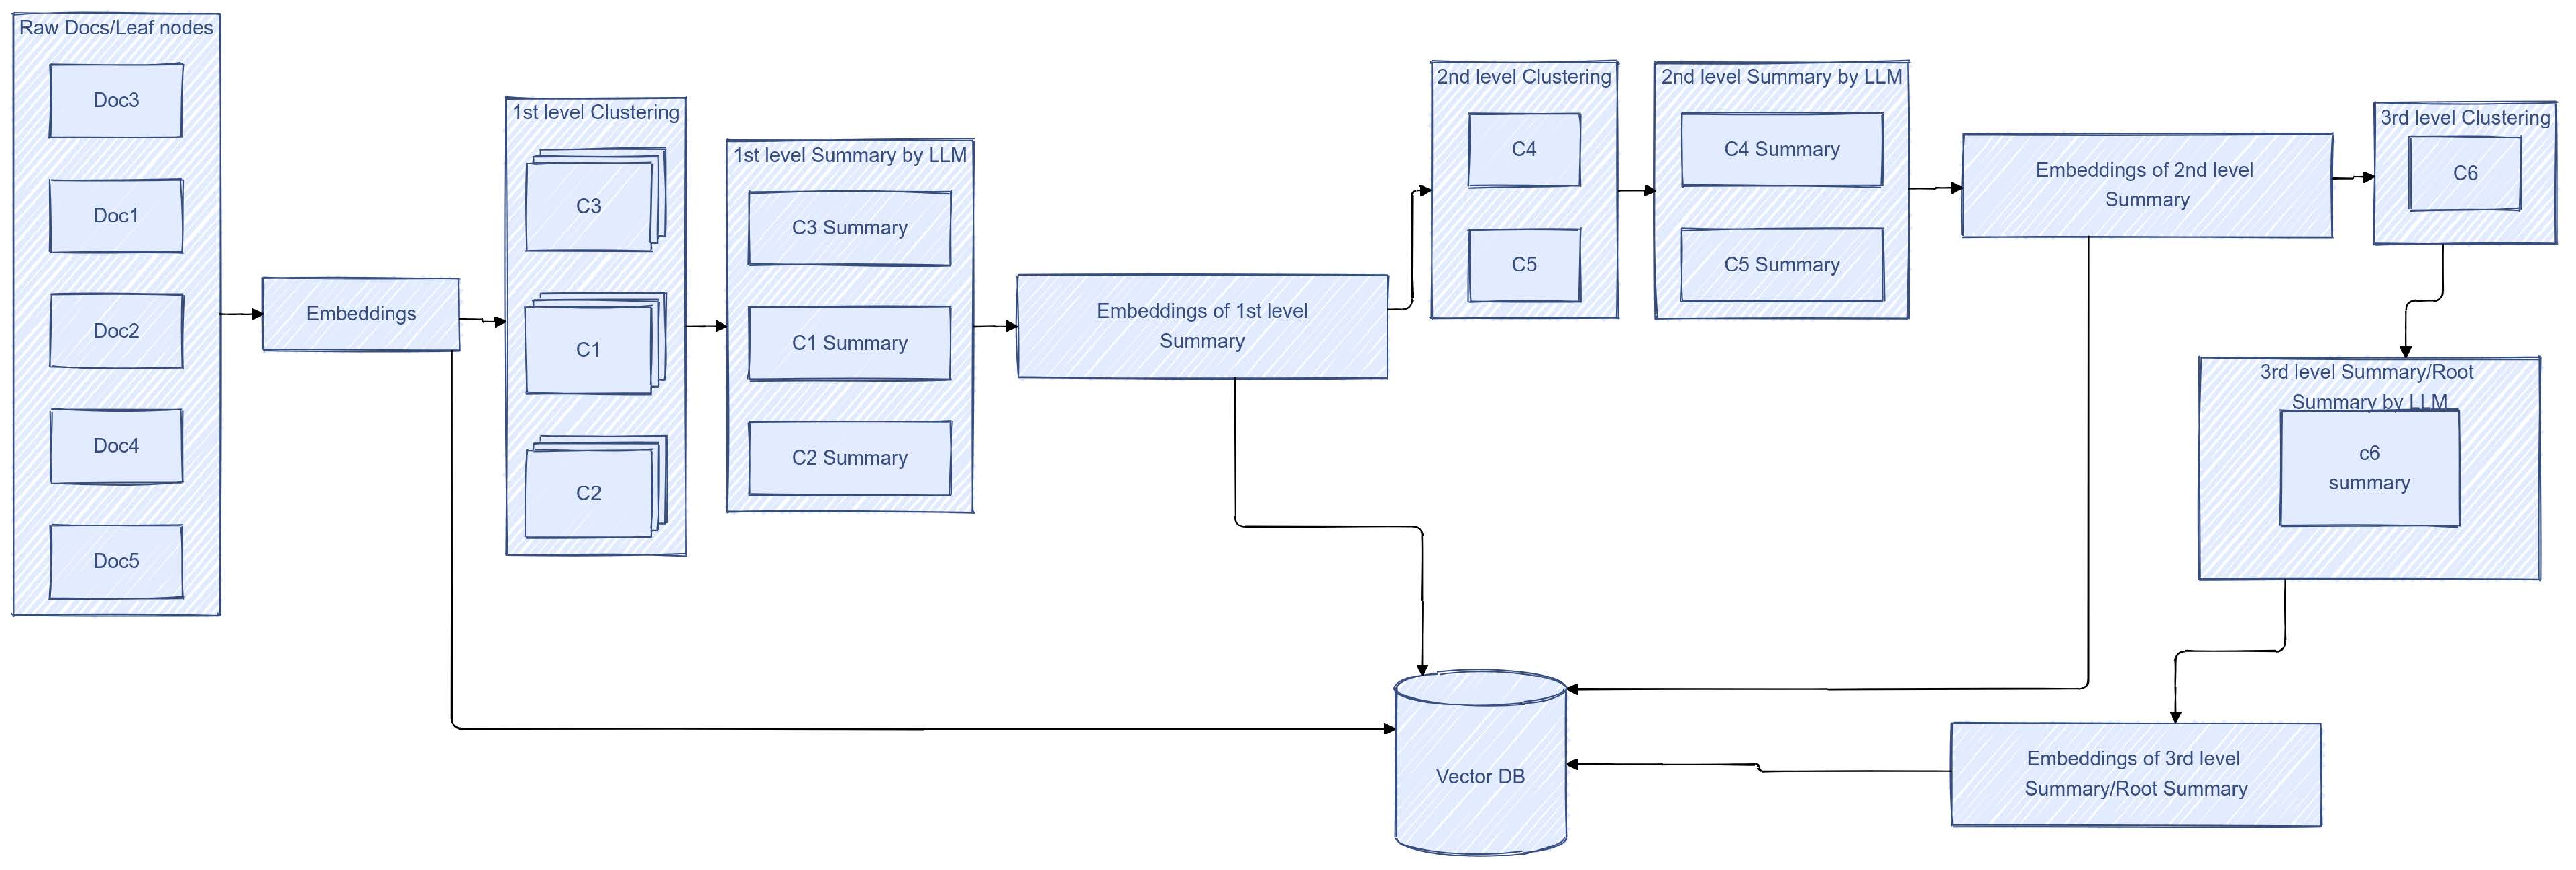
\includegraphics[width=\linewidth]{Raptor.pdf}
	\caption{Flow chart of RAPTOR processing of documents as integrated in MyRAG}
	\label{fig:raptor}
\end{figure}

\subsection{Pipeline Implementation}\label{subsec3.7}

The pipeline integrates the components described in \ref{subsec3.1}-\ref{subsec3.6} into a modular sequence. Documents are parsed and chunked (\ref{subsec3.1}), embedded (\ref{subsec3.2}), and stored in a vector database (\ref{subsec3.3}). Queries undergo a similar embedding process and are matched against these embeddings to retrieve top-$k$ relevant chunks. ColBERT reranking (\ref{subsec3.5}) or RAPTOR hierarchical retrieval (\ref{subsec3.6}) can be applied before generating the final response with an LLM (\ref{subsec3.4}). It  ensures easy configuration, reproducibility, and extension, while enabling direct comparisons across different pipeline configurations.


\section{Evaluations and Results}\label{sec4}

%----------------- Datasets -----------------%
\subsection{Datasets}\label{sec4.1}

\textbf{1. Hugging Face Document QA Evaluation Dataset(HF QA):}

The \textit{huggingface\_doc\_qa\_eval} dataset is a synthetic dataset consisting of question-answer pairs extracted from the markdown files of the Hugging Face repository on GitHub. It is specifically designed for evaluating Retrieval-Augmented Generation (RAG) systems \cite{huggingface2024docqa}. The dataset contains a total of 65 unique questions, each paired with its corresponding answer, context, and source document path.

Out of the ten available columns in the dataset, the following four were used for evaluation:
\begin{itemize}
    \item \textbf{Context:} The content retrieved from the corresponding markdown file.
    \item \textbf{Question:} The query posed to the system.
    \item \textbf{Answer:} The ideal answer to the question.
    \item \textbf{Source\_doc:} The path to the markdown file in the Hugging Face GitHub repository.
\end{itemize}

The dataset was loaded in Parquet format using the Hugging Face API. Each question-answer pair was derived from a unique markdown file, ensuring there was no overlap in the source documents. This design allows for precise evaluation of RAG systems in retrieving relevant content from specific documents.

\textbf{2. BioASQ11 Challenge Dataset(BioASQ):}

The \textit{BioASQ11} dataset was obtained from the 2023 iteration of the BioASQ challenge, specifically training set (11b) of Task Set B for biomedical question answering \cite{bioasq2023}. The training set (11b) consists of a total of 4,719 questions, each provided with gold-standard annotations, including concepts, article URLs, snippets, RDF triples, "exact" answers, and "ideal" answers.

Due to the size of the dataset and restrictions on accessing articles from certain URLs, a filtering process was applied:
\begin{itemize}
    \item Articles that required credentials for access were excluded.
    \item To comply with server limitations on large-scale downloads, only a subset of 13 questions with 42 associated PDFs was retained for the evaluation.
\end{itemize}

For each retained question, answers are derived from 1 to 7 different PDFs. To facilitate evaluation, a CSV file was created for this filtered questions with the following columns:
\begin{itemize}
    \item \textbf{Question ID:} A unique identifier for each question.
    \item \textbf{Question:} The query posed.
    \item \textbf{Ideal Answer:} The gold-standard answer for the question.
    \item \textbf{Download Link:} The URL for downloading the article PDF.
    \item \textbf{PDF Reference:} The specific reference to the PDFs used for the answer.
\end{itemize}

A web scraping script was developed to retrieve PDF file URLs from the provided article links. This processed dataset enables systematic evaluation of retrieval accuracy and relevance in biomedical contexts.

\subsection{TOP-K Retrieval Accuracies}\label{sec4.2}

Retrieval accuracy for each embedding model is evaluated using a standard top-$k$ retrieval metric. Given $N$ queries, let $\text{retrieved}_i@k$ denote the set of top-$k$ retrieved chunks document ids for the $i$-th query, and let $\text{relevant}_i$ represent the set of relevant document ids for that query. The top-$k$ retrieval accuracy, $\text{Accuracy@k}$, is computed as follows:

\begin{equation}
\text{Accuracy@k} = \frac{1}{N} \sum_{i=1}^{N} 
    \begin{cases}
      \mathbbm{1}(\exists d \in \text{retrieved}_i@k : d \in \text{relevant}_i), & \text{if } |\text{relevant}_i| = 1 \text{ or } k = 1 \\[6pt]
      \frac{|\text{retrieved}_i@k \cap \text{relevant}_i|}{\min(k, |\text{relevant}_i|)}, & \text{otherwise}
    \end{cases}
\end{equation}

The evaluations are conducted on both the BioASQ and Hugging Face Document QA datasets(HF QA). All runs use the common retrieval parameters shown in Table~\ref{table:retrieval_params}. Each query is processed using a given embedding model, and the resulting top-$k$ candidates are examined according to the equation above.

\begin{table}[h]
\centering
\begin{tabular}{|p{4cm}|p{8cm}|}
\hline
\textbf{Retrieval Parameter} & \textbf{Value} \\
\hline
Chunk Size & 4000 tokens \\
Chunk Overlap & 200 tokens \\
Top-$k$ & 1,2,3,4,5,7,8,10 \\
Query Instruction for query embedding generation & \textbf{NV-Embed-v2}: "Instruct: Given a question, retrieve passages that answer the question. Query:" \\ 
~ & \textbf{stella\_en\_1.5B\_v5 }: "Instruct: Given a web search query, retrieve relevant passages that answer the query. Query:" \\
~ & no instructions were used for queries embedding with  other embedding models\\
\hline
\end{tabular}
\caption{Common retrieval parameters and instructions used across experiments.}
\label{table:retrieval_params}
\end{table}


\begin{table}[h]
\centering
\begin{tabular}{|l|c|c|c|}
\hline
\textbf{Embedding Model} & \textbf{Quantization} & \textbf{Size (GB)} & \textbf{Parameters (M)} \\ \hline
mxbai-embed-large-v1      & None   & 1.25 & 335.14 \\ \hline
stella\_en\_1.5B\_v5 (8-bit) & 8-bit & 3.48 & 1543.27 \\ \hline
stella\_en\_1.5B\_v5         & None  & 9.25 & 1543.27 \\ \hline
NV-Embed-v2 (8-bit)       & 8-bit & 7.44 & 7851.02 \\ \hline
all-MiniLM-L6-v2          & None  & 0.08 & 22.71 \\ \hline
titan-embed-text-v2       & Unknown & Unknown & Unknown \\ \hline
\end{tabular}
\caption{Specifications of embedding models evaluated.}
\label{table:model_specs}
\end{table}


Table~\ref{table:model_specs} presents the model specifications. The \texttt{mxbai-embed-large-v1} model is extremely resource-efficient and still provides competitive performance, making it suitable for environments with limited computational capacity. In contrast, \texttt{NV-Embed-v2 (8-bit)} is notably larger, yet still manageable due to quantization, and it achieves performance comparable to much larger models. The \texttt{stella\_en\_1.5B\_v5} model is larger and performs slightly better than \texttt{NV-Embed-v2 (8-bit)}, but at the cost of higher resource usage. Despite its closed-source nature and unknown parameters, \texttt{titan-embed-text-v2} does not surpass the best open source embedding models. The \texttt{all-MiniLM-L6-v2} model, while very lightweight, trails behind the top performers.

\begin{table}[h]
\centering
\small
\begin{tabular}{l l c c c c c c c c}
\hline
\textbf{Model} & \textbf{Dataset} & \textbf{k=1} & \textbf{k=2} & \textbf{k=3} & \textbf{k=4} & \textbf{k=5} & \textbf{k=7} & \textbf{k=8} & \textbf{k=10} \\
\hline
\multirow{2}{*}{NV-Embed-v2 (8-bit)} 
 & BioASQ & 1.00 & 0.85 & 0.79 & 0.76 & 0.77 & 0.79 & 0.80 & 0.80 \\
 & HF QA  & 0.91 & 0.94 & 0.98 & 0.98 & 0.98 & 1.00 & 1.00 & 1.00 \\
\hline
\multirow{2}{*}{all-MiniLM-L6-v2} 
 & BioASQ & 0.62 & 0.58 & 0.51 & 0.47 & 0.57 & 0.54 & 0.57 & 0.61 \\
 & HF QA  & 0.58 & 0.66 & 0.72 & 0.74 & 0.77 & 0.80 & 0.82 & 0.83 \\
\hline
\multirow{2}{*}{mxbai-embed-large-v1} 
 & BioASQ & 1.00 & 0.92 & 0.77 & 0.70 & 0.74 & 0.77 & 0.79 & 0.79 \\
 & HF QA  & 0.95 & 0.95 & 0.95 & 0.95 & 0.95 & 0.98 & 0.98 & 0.98 \\
\hline
\multirow{2}{*}{stella\_en\_1.5B\_v5} 
 & BioASQ & 1.00 & 0.73 & 0.72 & 0.71 & 0.72 & 0.74 & 0.75 & 0.79 \\
 & HF QA  & 0.95 & 0.98 & 0.98 & 0.98 & 1.00 & 1.00 & 1.00 & 1.00 \\
\hline
\multirow{2}{*}{stella\_en\_1.5B\_v5 (8-bit)} 
 & BioASQ & 0.31 & 0.42 & 0.64 & 0.66 & 0.68 & 0.74 & 0.74 & 0.78 \\
 & HF QA  & 0.88 & 0.91 & 0.91 & 0.91 & 0.92 & 0.94 & 0.94 & 0.94 \\
\hline
\multirow{2}{*}{titan-embed-text-v2} 
 & BioASQ & 1.00 & 0.81 & 0.69 & 0.67 & 0.69 & 0.67 & 0.68 & 0.73 \\
 & HF QA  & 0.89 & 0.91 & 0.95 & 0.97 & 0.98 & 0.98 & 0.98 & 0.98 \\
\hline
\end{tabular}
\caption{Top-$k$ retrieval accuracy for standard RAG. All evaluations are performed with the parameters and instructions listed in Table~\ref{table:retrieval_params}.}
\label{table:standard_rag_results}
\end{table}

Table~\ref{table:standard_rag_results} shows the top-$k$ retrieval accuracy under standard RAG (no reranking). It can be observed that \texttt{NV-Embed-v2 (8-bit)}, \texttt{mxbai-embed-large-v1}, and \texttt{stella\_en\_1.5B\_v5} achieve strong accuracy scores. Although \texttt{NV-Embed-v2 (8-bit)} is large, quantization allows it to be memory-efficient. The \texttt{mxbai-embed-large-v1} model stands out as both lightweight and high-performing, while \texttt{all-MiniLM-L6-v2} remains light weight but lags in accuracy. The closed-source \texttt{titan-embed-text-v2} does not outperform the open source models.



ColBERT v2.0 reranking is then introduced to refine the top-K results from an initial retrieval of 15 chunks. The reranking parameters used are shown in Table~\ref{table:rerank_params}, and Table~\ref{table:rerank_results} presents the corresponding accuracy scores. The ColBERT reranking model, with a size of only 0.41 GB and 110M parameters, quickly rescored candidates without significant overhead.

\begin{table}[h]
\centering
\begin{tabular}{|p{4cm}|p{8cm}|}
\hline
\textbf{Reranking Parameter} & \textbf{Value} \\
\hline
Initial Retrieval Top $k$ & 15 \\
Reranking Top $k$ & 1,2,3,4,5,7,8,10 \\
Chunk Size & 4000 tokens \\
Chunk Overlap & 200 tokens \\
Query Instruction for query embedding generation & \textbf{NV-Embed-v2}: "Instruct: Given a question, retrieve passages that answer the question. Query:" \\ 
~ & \textbf{stella\_en\_1.5B\_v5 }: "Instruct: Given a web search query, retrieve relevant passages that answer the query. Query:" \\
~ & no instructions were used for queries embedding with all other embedding models including reranking ColBERT v2.0 embedding model \\
\hline
\end{tabular}
\caption{Parameters used for experiments involving ColBERT v2.0 Reranking.}
\label{table:rerank_params}
\end{table}

\begin{table}[h]
\centering
\small
\begin{tabular}{l l c c c c c c c c}
\hline
\textbf{Model} & \textbf{Dataset} & \textbf{k=1} & \textbf{k=2} & \textbf{k=3} & \textbf{k=4} & \textbf{k=5} & \textbf{k=7} & \textbf{k=8} & \textbf{k=10} \\
\hline
\multirow{2}{*}{NV-Embed-v2 (8-bit)} 
 & BioASQ & 1.00 & 0.81 & 0.74 & 0.77 & 0.78 & 0.80 & 0.80 & 0.82 \\
 & HF QA  & 0.97 & 0.98 & 0.98 & 0.98 & 0.98 & 0.98 & 1.00 & 1.00 \\
\hline
\multirow{2}{*}{all-MiniLM-L6-v2} 
 & BioASQ & 0.85 & 0.77 & 0.72 & 0.67 & 0.69 & 0.72 & 0.72 & 0.73 \\
 & HF QA  & 0.88 & 0.89 & 0.89 & 0.89 & 0.91 & 0.91 & 0.91 & 0.91 \\
\hline
\multirow{2}{*}{mxbai-embed-large-v1} 
 & BioASQ & 1.00 & 0.88 & 0.77 & 0.73 & 0.74 & 0.80 & 0.82 & 0.82 \\
 & HF QA  & 0.92 & 0.97 & 0.97 & 0.98 & 0.98 & 0.98 & 0.98 & 0.98 \\
\hline
\multirow{2}{*}{stella\_en\_1.5B\_v5} 
 & BioASQ & 1.00 & 0.85 & 0.72 & 0.67 & 0.73 & 0.79 & 0.79 & 0.79 \\
 & HF QA  & 0.95 & 0.98 & 0.98 & 0.98 & 0.98 & 0.98 & 0.98 & 1.00 \\
\hline
\multirow{2}{*}{stella\_en\_1.5B\_v5 (8-bit)} 
 & BioASQ & 0.92 & 0.81 & 0.72 & 0.67 & 0.68 & 0.69 & 0.70 & 0.72 \\
 & HF QA  & 0.77 & 0.77 & 0.77 & 0.77 & 0.78 & 0.78 & 0.78 & 0.82 \\
\hline
\multirow{2}{*}{titan-embed-text-v2} 
 & BioASQ & 1.00 & 0.85 & 0.74 & 0.71 & 0.73 & 0.75 & 0.77 & 0.79 \\
 & HF QA  & 0.92 & 0.95 & 0.95 & 0.95 & 0.95 & 0.95 & 0.97 & 0.98 \\
\hline
\end{tabular}
\caption{Top-$k$ retrieval accuracy after ColBERT reranking.}
\label{table:rerank_results}
\end{table}

ColBERT reranking generally improves performance for models that had weaker initial retrieval results. For instance, \texttt{all-MiniLM-L6-v2} and \texttt{titan-embed-text-v2} show notable gains, indicating that fine-grained token-level scoring helps surface more relevant candidates at top ranks. For strong models like \texttt{NV-Embed-v2 (8-bit)}, reranking raises the HF QA $k=1$ accuracy from 0.91 to 0.97, but the gains diminish at higher $k$ values, suggesting that reranking is most beneficial for improving the very light weight models.

The RAPTOR-based retriever is not included in these top-$k$ evaluations as it involves hierarchical summaries from multiple documents that complicate direct comparison to standard retrieval methods. Future iterations will incorporate RAPTOR retrieval accuracies, enabling comparisons across the full spectrum of retrieval strategies.

\subsection{RAG Evaluation}\label{subsec4.3}

The end-to-end effectiveness of the Retrieval-Augmented Generation (RAG) pipeline is assessed by integrating the retrieved document chunks into a Large Language Model (LLM) for final answer generation. All experiments described here use Anthropic's Claude 3.5 Sonnet (20240620-v1) model accessed through AWS Bedrock. Preliminary tests with Meta-Llama-3-8B-Instruct (8-bit) indicated insufficient answer quality and limited computational resources, so the evaluations focus exclusively on the Claude.

Table~\ref{table:rag_eval_standard} presents the performance of standard RAG across each embedding model. The system message and generation configuration remain consistent in all experiments, as defined in the evaluation configuration files. This generation configuration ensures that the same input produces the same deterministic response under identical conditions. The parameters are:

\begin{itemize}
    \item System Message:
\begin{verbatim}
You are an AI assistant that provides accurate and helpful answers
based on the given context. Your responses should be:
1. Focused on the provided context
2. Clear and concise
3. Accurate and relevant to the question
4. Based only on the information given
\end{verbatim}

    \item Generation Config:
\begin{verbatim}
max_tokens: 512
temperature: 0.1
top_k: 50
top_p: 0.9
anthropic_version: bedrock-2023-05-31
\end{verbatim}
\end{itemize}

The standard RAG evaluation uses $TOP\ k\ chunk\ retrieved =5$, $chunk\_size=4000$, $chunk\_overlap=200$ and Query Instructions  same as done in top k retrieval.

\begin{table}[h]
\centering
\small
\begin{tabular}{l l c c c c c c c}
\hline
\textbf{Embedding Model} & \textbf{Dataset} & \textbf{Total} & \textbf{Correct} & \textbf{Incorrect} & \textbf{Partial} & \textbf{Correct (\%)} \\
\hline
\multirow{2}{*}{NV-Embed-v2 (8-bit)} 
 & HF QA  & 65 & 64 & 1 & 0 & 98.46 \\
 & BioASQ & 13 & 9  & 1 & 3 & 69.23 \\
\hline
\multirow{2}{*}{all-MiniLM-L6-v2} 
 & HF QA  & 65 & 50 & 15 & 0 & 76.92 \\
 & BioASQ & 13 & 6  & 3  & 4 & 46.15 \\
\hline
\multirow{2}{*}{mxbai-embed-large-v1} 
 & HF QA  & 65 & 62 & 3 & 0 & 95.38 \\
 & BioASQ & 13 & 8  & 1 & 4 & 61.54 \\
\hline
\multirow{2}{*}{stella\_en\_1.5B\_v5} 
 & HF QA  & 65 & 64 & 1 & 0 & 98.46 \\
 & BioASQ & 13 & 9  & 0 & 4 & 69.23 \\
\hline
\multirow{2}{*}{titan-embed-text-v2} 
 & HF QA  & 65 & 63 & 2 & 0 & 96.92 \\
 & BioASQ & 13 & 8  & 0 & 5 & 61.54 \\
\hline
\end{tabular}
\caption{End-to-end RAG performance under standard retrieval conditions.}
\label{table:rag_eval_standard}
\end{table}

Under standard RAG, both NV-Embed-v2 (8-bit) and Stella EN 1.5B v5 achieve high correctness percentages in HF QA, exceeding 98\% correct responses. The mxbai-embed-large-v1 and titan-embed-text-v2 models also perform well, surpassing 95\% correctness on HF QA. The all-MiniLM-L6-v2 model yields lower correctness, especially on BioASQ. For more specialized domains like BioASQ, performance generally declines compared to HF QA (each answer from a single document), reflecting the increased difficulty of biomedical questions from multiple documents.

Next, Table~\ref{table:rag_eval_rerank} presents the results of standard RAG augmented with ColBERT reranking. The reranking configuration uses $max\_k=15$ for initial retrieval and $rereank\_max\_k=5$ for the final selection. All other parameters, including the generation configuration, remain consistent. ColBERT reranking did not significantly change correctness percentages for most models. While token-level reranking refines top document selection, it does not necessarily translate into substantially improved final answer correctness. The all-MiniLM-L6-v2 model shows some gains on HF QA, improving from 76.92\% to 89.23\%, but on BioASQ performance declines further, highlighting the complexity of biomedical queries.

\begin{table}[h]
\centering
\small
\begin{tabular}{l l c c c c c}
\hline
\textbf{Embedding Model} & \textbf{Dataset} & \textbf{Total} & \textbf{Correct} & \textbf{Incorrect} & \textbf{Partial} & \textbf{Correct (\%)} \\
\hline
\multirow{2}{*}{NV-Embed-v2 (8-bit)} 
 & HF QA  & 65 & 63 & 2 & 0 & 96.92 \\
 & BioASQ & 13 & 8  & 0 & 5 & 61.54 \\
\hline
\multirow{2}{*}{all-MiniLM-L6-v2} 
 & HF QA  & 65 & 58 & 7 & 0 & 89.23 \\
 & BioASQ & 13 & 5  & 3 & 5 & 38.46 \\
\hline
\multirow{2}{*}{mxbai-embed-large-v1} 
 & HF QA  & 65 & 63 & 2 & 0 & 96.92 \\
 & BioASQ & 13 & 8  & 0 & 5 & 61.54 \\
\hline
\multirow{2}{*}{stella\_en\_1.5B\_v5} 
 & HF QA  & 65 & 63 & 2 & 0 & 96.92 \\
 & BioASQ & 13 & 8  & 0 & 5 & 61.54 \\
\hline
\multirow{2}{*}{titan-embed-text-v2} 
 & HF QA  & 65 & 62 & 3 & 0 & 95.38 \\
 & BioASQ & 13 & 8  & 0 & 5 & 61.54 \\
\hline
\end{tabular}
\caption{End-to-end RAG performance with ColBERT reranking.}
\label{table:rag_eval_rerank}
\end{table}

Finally, Table~\ref{table:rag_eval_raptor} reports the results when using the RAPTOR hierarchical summarization-based retrieval architecture. RAPTOR uses a summarization template designed to handle multiple documents effectively:

\begin{verbatim}
Here is a sub-set of documents. 
Give a detailed summary of the content provided.

Documents:
\end{verbatim}


\begin{table}[h]
\centering
\small
\begin{tabular}{l l c c c c c}
\hline
\textbf{Embedding Model} & \textbf{Dataset} & \textbf{Total} & \textbf{Correct} & \textbf{Incorrect} & \textbf{Partial} & \textbf{Correct (\%)} \\
\hline
\multirow{2}{*}{mxbai-embed-large-v1} 
 & HF QA  & 65 & 64 & 1 & 0 & 98.46 \\
 & BioASQ & 13 & 9  & 1 & 3 & 69.23 \\
\hline
\multirow{2}{*}{stella\_en\_1.5B\_v5} 
 & HF QA  & 65 & 65 & 0 & 0 & 100.00 \\
 & BioASQ & 13 & 10 & 0 & 3 & 76.92 \\
\hline
\end{tabular}
\caption{End-to-end RAG performance using the RAPTOR architecture.}
\label{table:rag_eval_raptor}
\end{table}

RAPTOR excels at managing complex, multi-document queries. As shown in Table~\ref{table:rag_eval_raptor}, Stella EN 1.5B v5 with RAPTOR achieves perfect correctness (100\%) on HF QA and 76.92\% correctness on BioASQ, outperforming both the standard and reranked RAG configurations. The mxbai-embed-large-v1 model also shows improvement under RAPTOR. Due to computational resource limitations and maximum token constraints, other embedding models, could not be tested in this RAPTOR architecture. Nevertheless, the RAPTOR-based approach demonstrates promising gains in challenging domains like biomedical QA, where detailed reasoning and synthesis from multiple sources are crucial.

%----------------- Challenges and Future Work -----------------%
\section{Challenges and Future Work}\label{sec5}
\begin{itemize}
    \item \textbf{Evaluation Metrics:} Current retriever evaluation focuses on document-level accuracy. Future work includes more fine-grained evaluation (e.g., chunk level), automated scoring methods for retriever, and domain expert assessments of entire QA RAG to better understand retrieval quality in specialized domains.
    
    \item \textbf{Document Parsing:} MyRAG currently processes textual data. Extending it to multimodal inputs (PDFs with figures, images, or even audio transcripts) would demand integrating vision and ASR models, enabling comprehensive retrieval across diverse data formats.
    
    \item \textbf{Multi-agent Systems:} A future direction involves multi-agent LLM architectures where one agent refines user queries and another specializes in retrieval. Iterative query clarification and refinement would ensure that only the most relevant information is retrieved for the LLM to answer.
\end{itemize}

%----------------- Conclusion -----------------%
\section{Conclusion}\label{sec6}

This work introduced MyRAG, an open source code for systematically comparing a variety of Retrieval-Augmented Generation (RAG) architectures, embedding models, vector databases, and retrieval enhancement techniques. The experiments demonstrated that even lightweight embedding models, such as mxbai-embed-large-v1, can perform competitively in top-$k$ retrieval accuracy, offering efficient solutions suitable for resource-constrained environments. While larger models like NV-Embed-v2 (8-bit) and Stella EN 1.5B v5 provided slightly better retrieval accuracy, the differences were marginal. ColBERT reranking generally improved retrieval accuracy for models with weaker initial performance, though its benefits diminished at higher values of $k$. This suggests that while token-level reranking can refine top candidates, it may not guarantee significant gains across broader retrieval sets.

The end-to-end RAG evaluation provided further insight into how embedding models and retrieval methods influence final answer quality. Standard RAG delivered strong correctness on simpler tasks, while more complex and domain-specific questions, such as those from BioASQ, proved more challenging. ColBERT reranking led to moderate improvements in certain cases (e.g., all-MiniLM-L6-v2 on HF QA), but did not universally enhance final answer accuracy. In contrast, the RAPTOR hierarchical retrieval architecture offered substantial improvements for difficult, multi-document BioASQ queries.

These findings highlight the importance of selecting the right combination of embedding model, retrieval strategy, and architecture to achieve optimal RAG performance. Future work will focus on more granular retrieval evaluations, integrating multimodal data, and exploring multi-agent LLM architectures. By continually refining RAG pipelines and incorporating new advancements, MyRAG aims to serve as a versatile and evolving platform for building more effective and efficient retrieval-augmented systems.

\paragraph{Acknowledgments:} The author extends sincere gratitude to Abdygulov Timur for his guidance in understanding and developing the standard RAG, ColBERT, and RAPTOR architectures, as well as for assisting in preparing the BioASQ dataset for evaluation. The author also thanks Professor Amir H. Jafari for helping understand RAG concept, sharing literature related to RAG, introducing the BioASQ dataset,  and for his impactful NLP and Deep Learning courses, which greatly contributed to the successful implementation of the methods described in this work.

\bibliography{sn-bibliography}% common bib file
%% if required, the content of .bbl file can be included here once bbl is generated
%%\input sn-article.bbl


\end{document}
